% This is based on the LLNCS.DEM the demonstration file of
% the LaTeX macro package from Springer-Verlag
% for Lecture Notes in Computer Science,
% version 2.4 for LaTeX2e as of 16. April 2010
%
% See http://www.springer.com/computer/lncs/lncs+authors?SGWID=0-40209-0-0-0
% for the full guidelines.
%

\documentclass{llncs}

\usepackage{mathtools}

\usepackage{fancyhdr} 
\cfoot{\thepage}
\pagestyle{fancy}  


\begin{document}

\title{STAT 538 Paper Review \\ Weisfeiler-Lehman Graph Kernels}
%
\titlerunning{Hamiltonian Mechanics}  % abbreviated title (for running head)
%                                     also used for the TOC unless
%                                     \toctitle is used
%
\author{Jinyu Xia}
\institute{\email{jinyuxia@uw.edu}}

\maketitle              % typeset the title of the contribution

\begin{abstract}
This is the review report of Weisfeiler-Lehman Graph Kernels by Shervashidze et al. The report consists of two major sections. The first section includes the definition of three Weisfeiler-Lehman graph kernels the paper discussed, and a proof of their positive semi-definiteness. The second part presents regenerated experiment evaluation of the classification accuracy and runtime of Weisfeiler-Lehman graph kernels. 
\keywords{graph kernels, graph classification, Weisfeiler-Lehman algorithm, similarity measures for graphs}
\end{abstract}

%
\section{The General Weisfeiler-Lehman Kernels Framework}
%

\begin{definition} 

Let $k$ be any kernel for graphs, that we will call the base kernel. Then the Weisfeiler-Lehman kernel with $h$ iteration with the base kernel $k$ is defined as

\begin{equation}
  k_{wl}^{(h)}(G, G^{\prime}) = k(G_0, G_0^{\prime}) + k(G_1, G_1^{\prime}) + ... + k(G_h, G_h^{\prime})
  \label{eq:one}
\end{equation}

where $h$ is the number of Weisfeiler-Lehman iterations and $\{G_0,..., G_h\}$ and $\{G_0^{\prime},..., G_h^{\prime}\}$ are the Weisfeiler-Lehman sequences of $G$ and $G^{\prime}$ respectively. 

\end{definition}

\begin{theorem} In Weisfeiler-Lehman kernel (\ref{eq:one}), if the base kernel $k$ is positive semidefinite, then the corresponding Weisfeiler-Lehman kernel $k_{wl}^{(h)}$ is positive semidefinite. 
\end{theorem}


%
\begin{proof}

Let $\phi$ be the feature mapping corresponding to the kernel $k$: 

\begin{equation}
k(G_i, G_i^{\prime}) = \langle \phi(G_i), \phi(G_i^{\prime}) \rangle
\end{equation}

Define $\psi(G)$ as $\phi(r^{i}(G))$. Then we have 
\begin{equation}
k(G_i, G_i^{\prime}) = k(r^i (G), r^i (G^{\prime})) = \langle \phi(r^i (G)), \phi( r^i (G^{\prime})) \rangle = \langle \psi(G), \psi(G^{\prime}) \rangle
\end{equation}
Hence $k$ is a kernel on $G$ and $G^{\prime}$ and $k_{wl}^{(h)}$ is positive semidefinite as a sum of positive semidefinite kernels. 

\end{proof}



%
\section{Instances of Weisfeiler-Lehman Graph Kernels}
%
%
\subsection{The Weisfeiler-Lehman Subtree Kernel}
%

\begin{definition}
Let $G$ and $G^{\prime}$ be graphs. Define $\Sigma_i \subseteq \Sigma$ as the set of letters that occur as node labels at least once in $G$ and $G^{\prime}$ at the end of the i-th iteration of the Weisfeiler-Lehman algorithm. Let $\Sigma_0$ be the set of original node labels of $G$ and $G^{\prime}$. Assume all $\Sigma_i$ are pairwise disjoint. WLOG, assume that every $\Sigma_i = \{\sigma_{i1}, ..., \sigma_{i|\Sigma_i|} \}$ is ordered. Define a map $c_i: \{G, G^{\prime}) \times \Sigma_i \mapsto N$ such that $c_i(G, \sigma_{ij})$ is the number of occurrences of the letter $\sigma_{ij}$ in the graph $G$.  

The Weisfeiler-Lehman subtree kernel on two graphs $G$ and $G^{\prime}$ with $h$ iterations is defined as: 

\begin{equation}
k_{WLsubtree}^{(h)}(G, G^{\prime}) = \langle \phi_{WLsubtree}^{(h)} (G),  \phi_{WLsubtree}^{(h)} (G^{\prime})\rangle
\end{equation}

where 
\begin{align*}
\phi_{WLsubtree}^{(h)}(G) = (c_0(G, \sigma_{01}), ..., c_0(G, \sigma_{0 |\Sigma_0|}), ..., c_h(G, \sigma_{h1}),...,  c_h(G, \sigma_{h|\Sigma_h|})) 
\end{align*}
\begin{align*}
\phi_{WLsubtree}^{(h)}(G^{\prime}) = (c_0(G^{\prime}, \sigma_{01}, ..., c_0(G^{\prime}, \sigma_{0 |\Sigma_0|}), ..., c_h(G^{\prime}, \sigma_{h1}),...,  c_h(G^{\prime}, \sigma_{h|\Sigma_h|})
\end{align*}
\end{definition}

It can be showedthat the Weisfeiler-Lehman subtree kernel is a special case of the general Weisfeiler-Lahman kernel.

\begin{theorem}
Let the base kernel $k$ be a function counting pairs of matching node labels in two graphs: 

\begin{equation}
k(G, G^{\prime}) = \sum_{v \in V} \sum_{v^{\prime} \in V^{\prime}} \delta(l(v), l(v^{\prime}))
\end{equation}

where $\delta$ is the Dirac kernel, that is, it is 1 when its arguments are equal and 0 otherwise. Then $k_{WL}^{(h)}(G, G^{\prime}) = k_{WLsubtree}^{(h)} (G, G^{\prime})$ for all $G$, $G^{\prime}$.

\end{theorem}

\begin{proof}
It is easy to notice that for each $i \in \{0, 1, ..., h\}$ we have  
\begin{equation}
\sum_{v \in V} \sum_{v^{\prime} \in V^{\prime}} \delta(l_i(v), l_i^{\prime}(v^{\prime})) = \sum_{j=1}^{|\Sigma_i|} c_i(G, \sigma_{ij}) c_i(G^{\prime}, \sigma_{ij})
\end{equation}

Adding up these sums for all $i \in \{0, 1, ..., h\}$ gives us $k_{WL}^{(h)}(G, G^{\prime}) = k_{WLsubtree}^{(h)}(G, G^{\prime})$. The base kernel $k$ is positive semidefinite as sum of Dirac kernel. Thus, the Weisfeiler-Lehman Subtree Kernel is positive semidefinite. 

\end{proof}


%
\subsection{The Weisfeiler-Lehman Edge Kernel}
%

The Weisfeiler-Lehman edge kernel is another instance of the Weisfeiler-Lehman kernel framework. It is defined by  

\begin{equation}
k_{WLedge}^{(h)} = k_E(G_0, G_0^{\prime}) + k_E(G_1, G_1^{\prime}) + ... + k_E(G_h, G_h^{\prime})
\end{equation}

where the base kernel $k_E$ counts matching pairs of edges with identically labeled endpoints (incident nodes) in two graphs. In other words, the base kernel is defined as

\begin{equation}
k_E(G, G^{\prime}) = \langle \phi_E(G), \phi_E(G^{\prime}) \rangle
\end{equation}

where  $\phi_E(G)$ is a vector of number of occurences of pairs $(a, b)$, $a, b \in \Sigma$, which represent ordered labels of endpoints of an edge in $G$. Denoting $(a, b)$ and $(a^{\prime}, b^{\prime})$ the ordered labels of endpoints of edges $e$ and $e^{\prime}$ respectively, and $\delta$ the Dirac kernel, we can write $k_E$ as 

\begin{equation}
k_E(G, G^{\prime})  = \sum_{e\in E} \sum_{e^{\prime} \in E^{\prime}} \delta(a, a^{\prime}) \delta(b, b^{\prime})
\end{equation}

Therefore, Weisfeiler-Lehman Edge kernel is positive-semidefinite. 


%
\subsection{The Weisfeiler-Lehman Shortest Path Kernel}
%
The third instance of the general Weisfeiler-Lehman kernel is Weisfeiler-Lehman shortest path kernel, defined as 

\begin{equation}
k_{WL\ shortest\ path}^{(h)} = k_{SP}(G_0, G_0^{\prime}) + k_{SP}(G_1, G_1^{\prime}) + ... + k_{SP}(G_h, G_h^{\prime}) 
\end{equation}

whern fore the base kernel $k_{SP}(G, G^{\prime}) = \langle \phi_{SP}(G), \phi_{SP}(G^{\prime})\rangle$, $\phi_{SP}(G)$ is a vector whose components are numbers of occurrences of triplets of the form $(a, b, p)$ in $G$, where $a, b \in \Sigma$ are ordered endpoint labels of a shortest path and $p \in N_0$ is the shortest path length. In the following we'll prove the validity of shortest-path kernel.

An alternative form of Weisfeiler-Lehman shortest path kernel(Kondor and Borgwardt, 2008) is 

\begin{equation}
k_{SP}(G, G^{\prime}) = \sum_{e \in E} \sum_{e^{\prime} \in E^{\prime}} k_{walk}^{(1)} (e, e^{\prime})
\end{equation}

\begin{lemma}
The shortest-path graph kernel is positive definite.
\end{lemma}

\begin{proof}
The shortest-path kernel is simply a walk kernel run on a Floyd-transformed graph considering walks of length 1 only. First, we choose a positive definite kernel on nodes and a positive definite kernel on edges. We then define $k_{walk}^{(1)}$ on pairs of walks of length 1 as the product of kernels on nodes and edges encountered along the walk.

As a tensor product of node and edge kernels, $k_{walk}^{(1)}$ is positive definite. We then zero-extend $k_{walk}^{(1)}$ to the whole set of pairs of walks, setting kernel values for all walks with length $\neq 1$ to zero. This zero-extension preserves positive definiteness. The positive definiteness of the shortest-path kernel follows directly from its definition as a convolution kernel.
\end{proof}
%
\section{Kernel Based Method: Support Vector Classification}
%
For binary class data, given training vectors $\boldsymbol{x}_i \in R^n$, $i = 1,..., n$, and $\boldsymbol{y} \in R^n$ such that $y_i \in {1, -1}$, the loss function of kernel SVM is  

\begin{equation}
L[f]= \frac{1}{n} \sum_{i=1}^n max(0, 1 - f(x_i)y_i) + \frac{\lambda}{2} \|f\|^2 
\end{equation}

Since the SVM optimization problem can be expressed as  

\begin{equation}
J[f^*] = min_{f\in H} L[f] = min_{f \in H} \Psi(f(x_1), ..., f(x_n), \|f\|_H)
\end{equation}

where $H$ is the RKHS of $K$, and $\Psi$ is strictly increasing w.r.t to the last argument $\|f\|_H$. By representer theorem, the solution to SVC could be expressed as  

\begin{equation}
f^* = \sum_{i=1}^n \alpha_i k(x_i, \cdot)
\end{equation}

Thus, the object function of kernel SVC could be written as 

\begin{equation}
min_{\alpha \in R^n} \frac{1}{n}[max\{0, 1 - y_i (K\alpha_i)\}] + \frac{\lambda}{2} \alpha^T K \alpha
\end{equation}

However, we can directly perform functional gradient descent on the optimization problem of kernel SVM without invoking representer theorem. Let the cost function be $C_t = max\{0, 1 - f(x_i)y_i \}$. The gradient of $C_t$ is  

\begin{equation}
\nabla C_t = \left\{
                \begin{array}{ll}
                  0,  &1 - y_if(x_i) \leq 0 \\
                  C^{\prime}(F_{x_i}[f])(\nabla F_{x_i}[f]) = (-y_i)K(x_i, \cdot), \ \  & otherwise
                \end{array}
              \right.
\end{equation}

The general update rule would be 

\begin{equation}
f_{t+1} \leftarrow f_t(1 - \lambda \eta_t) - \eta_t C_t^{\prime}(F_{x_i}[f])K(x_i, \cdot)
\end{equation}

%
\section{Implementation}
%

I implemented these three Weisfeiler-Lehman subtree kernels mentioned above in python. Each kernel method has a key function that returns the similarity measures for two graphs. The kernel matrix $K$ is then computed based on it.  

There are two major parts when computing the kernel of two graphs. First of all, we need to conduct an initial count of either the node labels, edge or shortest path, depending on which instance of Weisfeiler-Lehman kernel graph is used. Then in the second part, the similarity of two graphs at i-th iteration is computed.   

The way long labels are compressed is by maintaining a map, of which the key is the string of long labels, and the value is the value of a counter that counts how many distinct labels has occurred so far.   

In addition, for Weisfeiler-Lehman shortest path kernel, Floyd-Warshall algorithm is implemented to compute the shortest path of two nodes in a graph.  

%
\section{Experiments}
%

\subsection{Runtime behavior of Weisfeiler-Lehman Subtree Kernel}

I examined the runtime behaviour of the non-recursion-version of Weisfeiler-Lehman subtree kernel. The runtime behaviour is assessed on randomly generated graphs with respect to four parameters: data set size $N$, graph size $n$, subtree height $h$ and graph desnity $c$. The value sets for four parameters were N in $\{10, 100, 1000\}$, $n$ in $\{100, 200, ..., 1000\}$, $\{2, 4, 8\}$, $\{0.1, 0.2, ..., 0.9\}$. When $N$ varied, the default values were 20 for $n$, 2 for $h$, 0.4 for $c$. Otherwise, the default values were 10 for $N$, 100 for $n$, 4 for $h$ and 0.4 for the graph desnity $c$. 3 out of 4 parameters were kept fixed at the defalut values while the fourth parameters varied. 


To achieve a certain level of node density $c$, I randomly select $c\frac{n(n-1)}{2}$ edges to be assigned as 1 in the adjacency matrix. One thing that of concern here is that I did not check if the edge assignment will lead to self-loop in the graph.  

The runtime in seconds for kernel matrix computation is shown in Figure \ref{1}. The runtime of my kernel matrix computations generally worse than the runtime reported in the paper, except the experiment for the effect of graph density on runtime (the plot on the bottom left) is quite similar to the plot in the paper. This indicates that there's room for complexity improvement in the graph kernel I implemented. One improvement could be store the neighbors of a node in a list so that we do not need to find the neighbors of a node from adjacency matrix each time. However, the good news is that the classification rate is consistent with (even better) than the classification rate reported in the paper. 

\begin{figure}[h]
\centering
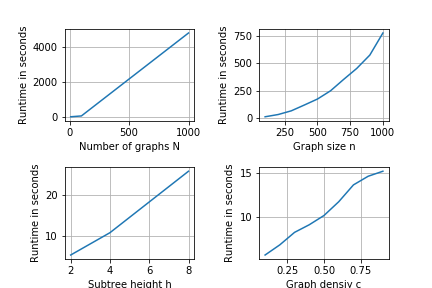
\includegraphics[width=\textwidth]{runtime}
\caption{Runtime in seconds for kernel matrix computation for Weisfeiler-Lehman subtree kernel (pairwise).}
\label{1}
\end{figure}



\subsection{Graph Classification}

\begin{figure}[!htb]
\minipage{0.32\textwidth}
  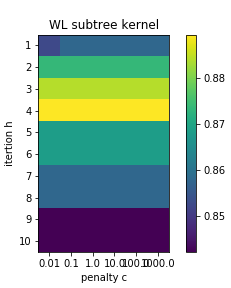
\includegraphics[width=\linewidth]{gk_sub}
  \label{fig:awesome_image1}
\endminipage\hfill
\minipage{0.32\textwidth}
  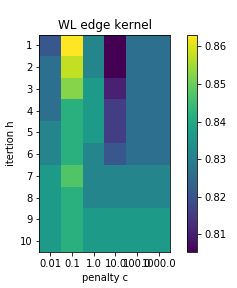
\includegraphics[width=\linewidth]{gk_edge}
  \label{fig:awesome_image2}
\endminipage\hfill
\minipage{0.32\textwidth}%
  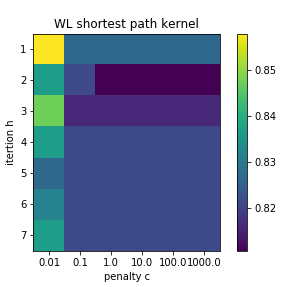
\includegraphics[width=\linewidth]{gk_sp}
  \label{fig:awesome_image3}
\endminipage
\caption{Grid search of hyperparamter $\lambda$ of SVM and number of iteration $h$, for three instances of Weisfeiler-Lehman Kernels, respectively. }
\end{figure}

I used MUTAG (Dehnath et al., 1991) as the data set when comparing the performance of the WL subtree kernel, the WL edge kernel, and the WL shortest path kernel. MUTAG is a data set of 188 mutagenic aromatic and heteroaromatic
nitro compounds labeled according to whether or not they have a mutagenic effect on the Gramnegative bacterium Salmonella typhimurium.  

The classification model used is Support Vector Machine Classification using LIBSVM. The model performance is evaluated by performing 10-fold cross-validation, using 9 folds for training and 1 for testing. Each experiment is repeated 10 times in order to exclude the random effects stemmed from fold assignment. 



There are two parameters need to be tunned, $h$ for WL kernel, and $c$ for SVC penalty. I did a grid search of $h \in \{ 1, 2, ..., 10\}$ for WL subtree and WL edge kernel, and a grid search of $h \in \{ 1, 2, ..., 7\}$ for WL shortest path kernel. The grid search of penalty $c$ is $\{ 0.01, 0.1, 1, 10, 100, 1000\}$, same for all three kernels. Note that when $h$ is set to be 0, the classification rate is around 0.6, regardless of the value of penalty $c$.  


\begin{table}[h!]
\centering
\begin{tabular}{ |p{3cm}||p{3cm}|p{3cm}|}
 \hline
 \multicolumn{3}{|c|}{MUTAG} \\
 \hline
	Method& Mean & Std\\ [0.5ex] 
 \hline
	WL subtree   & 86.68  & 7.71\\
 	WL edges     & 87.37  & 6.70  \\
 	WL shortes path & 83.42 & 7.64 \\ [1ex] 
 \hline
\end{tabular}
\caption{Prediction accuracy on graph classification (unit: \%)}
\label{table:1}
\end{table}

For WL subtree kernel, the penalty $c$ seems not matter so much in classification accuracy. The highest accuracy occurs when $h = 3, 4$.  For WL edge kernel, the optimal hyperparameter is $h = 1$ and $c = 0.1$.  For WL shortest path kernel, the optimal hyperparameter is $h = 1$ and $c = 0.01$. One thing that is not quite consistent with the paper result is that in the case of WL edge and WL shortest path kernel, the paper mentions that the values 2 and 3 of $h$ were almost always chosen by the cross-validation procedure, while in my experiment, $h = 1$ were chosen by cross-validation in the case of WL edge and WL shortest path kernel. It is worth mentioning that the prediction accuracies when $h$ is 2 or 3 are also quite competitive. 

To obtain the final prediction accuracy, I took the optimal parameters indicated by grid search, and repeat the classification given the optimal parameter 100 times. Each time the data was shuffled and split into a new training set (90\%) and test set (10\%). The accuracy is shown in Table \ref{table:1}. 

The average prediction accuracy I obtained for each graph kernel method is higher than the average prediction accuracy reported in the paper (Table 2, p.2558), while the standard deviation is larger than the standard deviation reported in the paper. I expected the inconsistency of experiment results come from the values of $h$, but overall the prediction accuracy results are quite satisfying. 



\section{Code}
The code for each WL subtree kernel, WL edge kernel, and WL shortest path kernel along with kernel-based classification methods and training methods are in $\texttt{WL\_subtree.ipynb}$, $\texttt{WL\_edge.ipynb}$, and $\texttt{WL\_ShortesPath.ipynb}$ respectively. The code for runtime experiment is in $\texttt{Runtime\_Experiment.ipynb}$. 

\end{document}
